%\documentclass[a4paper,
%%twocolumn
%]{article}
\documentclass[a4paper,9pt]{extarticle}

%%%%  Math
\usepackage{amsmath}
\DeclareMathOperator*{\argmin}{argmin}
\DeclareMathOperator*{\argmax}{argmax}
\newcommand*{\argminl}{\argmin\limits}
\newcommand*{\argmaxl}{\argmax\limits}

%%%%  Page margins
\usepackage{geometry}
%\geometry{left=25mm, right=20mm, top=30mm, bottom=20mm}
%\geometry{left=32mm, right=29mm, top=35mm, bottom=23mm}
\geometry{left=36mm, right=32mm, top=35mm, bottom=30mm}
%\geometry{left=15mm, right=15mm, top=25mm, bottom=20mm}
%\setlength{\columnsep}{4.5mm}

%%%% Configuration for plotting
%%%%%%  Math
\usepackage{amsmath}
\usepackage{amssymb}

%%%%%%  Tables
\usepackage{booktabs}
% \usepackage{longtable}
\usepackage{multirow}
\usepackage{pgfplotstable}
\DeclareMathVersion{sansserif}
\SetSymbolFont{operators}{sansserif}{OT1}{cmss}{m}{n}
\usepackage{siunitx} 
\sisetup{group-separator={,}, group-minimum-digits={3}, parse-numbers=false}
\usepackage{tabularx}
\usepackage{ltablex}
\usepackage{array}
\newcolumntype{P}{>{\raggedleft\arraybackslash}p{.2in}}
\newcommand*{\dsSizeInTable}{\footnotesize}
\newcommand*{\unitSizeInTable}{\scriptsize}
\newcommand*{\tableSize}{\small}

%%%%%%  Figures
\usepackage{caption}
\usepackage{subcaption}
\captionsetup[subfigure]{position=bottom, labelfont=bf, textfont=normalfont, singlelinecheck=off, justification=raggedright}

%%%%%%  Figures in same page as they're called in twocolumn
\usepackage{stfloats}

%%%%%%  Balance columns of the last page in twocolumn environment
\usepackage{balance}

%%%%%%  Equations numbering format
\makeatletter
\renewcommand{\theequation}{S\arabic{equation}}
\def\tagform@#1{\maketag@@@{\bfseries(Eq.~\ignorespaces#1\unskip\@@italiccorr)}}
\makeatother

%%%%%%  Marks
\usepackage{pifont}
\newcommand{\xmark}{\ding{53}\xspace}%
\newcommand{\fmark}{\ding{110}\xspace}%

%%%%%  Color
\usepackage{xcolor}
% \newcommand*{\highlight}[1]{\textcolor{red!90!black}{#1}}
%\usepackage{easyReview}
% \usepackage{soul}  % Highlight command \hl
% \DeclareRobustCommand{\highlight}[1]{{\sethlcolor{lightgray}\hl{#1}}}
% \newcommand*{\highlight}[1]{\tikz[baseline=(X.base)] \node[fill=lightgray] (X) {#1};}
\DeclareRobustCommand{\highlight}[1]{\colorbox{lightgray!30}{#1}}


%%%%%  Figures path
\usepackage{graphicx}
\graphicspath{{./fig/}}

%%%%%  Code styles
\usepackage{listings}
\lstset{
%	language=bash,
	basicstyle=\ttfamily,
	backgroundcolor=\color{black!5},
	commentstyle=\color{green!50!black},
	showstringspaces=false,
	numbers=left,
	numberstyle=\footnotesize\sffamily\color{gray!50},
	breaklines=true,
	mathescape=false %,
	% literate={\$}{{\$}}1
}
\lstdefinestyle{bash}{
	language=bash,
	basicstyle=\small\ttfamily,
}
\lstdefinestyle{cpp}{
	language=C++,
	basicstyle=\small\ttfamily,
}

%%%%%  Algorithms
\usepackage{algorithm}
\usepackage{algpseudocode}
\algnewcommand{\Inputs}[1]{%
  \State \textbf{Inputs:}
  \Statex \hspace*{\algorithmicindent}\parbox[t]{.8\linewidth}{\raggedright #1}
}
\renewcommand{\algorithmicrequire}{\textbf{Input:}}
\renewcommand{\algorithmicensure}{\textbf{Output:}}

%%%%%  Captions
\usepackage[figurename=Fig., tablename=Table, labelfont=bf, labelsep=period, font=small]{caption}
\renewcommand{\thefigure}{S\arabic{figure}}
\renewcommand{\thetable}{S\arabic{table}}

%%%%%  Links
\usepackage{hyperref}

%%%%%  Cites
\usepackage{cite}

%%%%%  Section, ... style
\usepackage{titlesec,titletoc}
\renewcommand*{\thesection}{S\arabic{section}}
\makeatletter
\renewcommand{\@seccntformat}[1]{%
	\ifcsname prefix@#1\endcsname
	\csname prefix@#1\endcsname
	\else
	\csname the#1\endcsname\quad
	\fi%
}
\newcommand\prefix@section{Note~\thesection\quad}
\makeatother
\titleformat*{\section}{\sffamily\Large\bfseries}
\titleformat*{\subsection}{\sffamily\large\bfseries}
\titleformat*{\subsubsection}{\sffamily\bfseries}
\titlecontents{section}[2.1em]{\addvspace{3mm}}{\bfseries\contentslabel{1.8em}}{\hspace*{-2.3em}}{\titlerule*[1pc]{}\bfseries\contentspage}
\dottedcontents{subsection}[4.9em]{}{2.8em}{1pc}

%%%%%  Line spacing
\usepackage{setspace}
\newcommand*{\defaultLineSpace}{\setstretch{1.15}}
\newcommand*{\codeLineSpace}{\setstretch{1.1}}
\newcommand*{\refLineSpace}{\setstretch{1}}

%%%%%  Handle spaces
\usepackage{xspace}

%%%%%  Trademark, registerd mark
\usepackage{textcomp}

%%%%%  User-defined commands
\newcommand*{\method}[1]{\text{#1}\xspace}
\newcommand*{\smashpp}   {\method{Smash++}}
\newcommand*{\gzip}      {\method{gzip}}
\newcommand*{\Gzip}      {\method{gzip}}
\newcommand*{\bzip}      {\method{bzip2}}
\newcommand*{\Bzip}      {\method{bzip2}}
\newcommand*{\mfcompress}{\method{MFCompress}}
\newcommand*{\Mfcompress}{\method{MFCompress}}
\newcommand*{\deliminate}{\method{DELIMINATE}}
\newcommand*{\Deliminate}{\method{DELIMINATE}}
\newcommand*{\fqzcomp}   {\method{fqzcomp}}
\newcommand*{\Fqzcomp}   {\method{Fqzcomp}}
\newcommand*{\quip}      {\method{Quip}}
\newcommand*{\Quip}      {\method{Quip}}
\newcommand*{\dsrc}      {\method{DSRC~2}}
\newcommand*{\Dsrc}      {\method{DSRC~2}}
\newcommand*{\fqc}       {\method{FQC}}
\newcommand*{\Fqc}       {\method{FQC}}
\newcommand*{\aes}		   {\method{AES}}
\newcommand*{\Aes}		   {\method{AES}}
\newcommand*{\aescrypt}  {\method{AES~Crypt}}
\newcommand*{\Aescrypt}  {\method{AES~Crypt}}
\newcommand*{\szip}      {\method{7zip}}
\newcommand*{\cmake}     {\method{cmake}}
\newcommand*{\Cmake}     {\method{Cmake}}
\newcommand*{\xs}		     {\method{XS}}
\newcommand*{\Xs}		     {\method{XS}}
\newcommand*{\goose}	   {\method{GOOSE}}
\newcommand*{\Goose}	   {\method{GOOSE}}
\newcommand*{\fasta}     {FASTA\xspace}
\newcommand*{\Fasta}     {FASTA\xspace}
\newcommand*{\fastq}     {FASTQ\xspace}
\newcommand*{\Fastq}     {FASTQ\xspace}
\newcommand*{\sam}       {SAM\xspace}
\newcommand*{\Sam}       {SAM\xspace}
\newcommand*{\bam}       {BAM\xspace}
\newcommand*{\Bam}       {BAM\xspace}
\newcommand*{\sambam}    {SAM/BAM\xspace}
\newcommand*{\Sambam}    {SAM/BAM\xspace}
\newcommand*{\vcf}       {VCF\xspace}
\newcommand*{\Vcf}       {VCF\xspace}
\newcommand*{\linux}     {Linux\xspace}
\newcommand*{\Linux}     {Linux\xspace}
\newcommand*{\windows}   {Windows\xspace}
\newcommand*{\Windows}   {Windows\xspace}
\newcommand*{\macos}     {macOS\xspace}
\newcommand*{\Macos}     {macOS\xspace}
\newcommand*{\xor}       {XOR\xspace}

\newcommand*{\sym}[1]{\text{#1}\xspace}
\newcommand*{\symA}      {\sym{A}}
\newcommand*{\symC}      {\sym{C}}
\newcommand*{\symG}      {\sym{G}}
\newcommand*{\symT}      {\sym{T}}
\newcommand*{\symN}      {\sym{N}}
\newcommand*{\symX}      {\sym{X}}

\newcommand*{\ascii}     {\mbox{ASCII}\xspace}

\newcommand*{\mono}[1]{\lstinline|#1|}
\newcommand*{\lang}[1]{\mono{#1}\xspace}
\newcommand*{\cpp}       {\lang{C++}}
\newcommand*{\bash}      {\lang{bash}}

%%%%%  User-defined environments
\lstnewenvironment{code}[1][]
	{\codeLineSpace\lstset{#1}\bgroup}
	{\egroup\defaultLineSpace}

%%%%  Headers and footers
\usepackage{fancyhdr}
\pagestyle{fancy}
\renewcommand{\sectionmark}[1]{\markright{Note~\thesection. #1}}
\renewcommand{\subsectionmark}[1]{\markright{\thesubsection. #1}}
\fancyhead{}    % clear all header fields
\fancyfoot{}    % clear all footer fields
\fancyhead[L]{\textsf{\nouppercase\rightmark}}
\fancyhead[R]{\thepage}
\setlength{\headsep}{20pt}


\begin{document}

% %%% Title page
% \begin{titlepage}
%   \centering
%   \vspace*{10mm}
%   % \includegraphics[width=2.8cm]{logo.png} \\[10mm]
%   \Large\textsc{Supplementary Material for} \\[5mm]
%   \huge\textbf{Smash++: finding rearrangements} \\[12mm]
%   \Large Morteza Hosseini\textsuperscript{1}, Diogo Pratas\textsuperscript{1,2}, Armando J. Pinho\textsuperscript{1} \\[6mm]
%   \normalsize \textsuperscript{1}IEETA/DETI, University of Aveiro, Portugal \\[1mm]
%   \textsuperscript{2}Department of Virology, University of Helsinki, Finland \\[4mm]
%   {\ttfamily\{seyedmorteza,pratas,ap\}@ua.pt}
  
%   \vspace{\fill}
%   \thispagestyle{empty}
%   \raggedright
%   \setstretch{1.2}
%   \normalsize\tableofcontents
% \end{titlepage}

% \defaultLineSpace    		%%% Line spacing

% \clearpage
% \section{GGA 18 compared to MGA 20}
% \begin{figure}[!h]
%   \centering
%   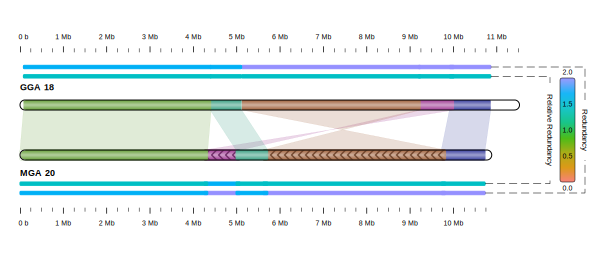
\includegraphics[width=.85\linewidth]{fig/GGA18_MGA20.pdf}
%   \caption{Pair-wise comparison of \textit{G.~gallus} chromosome~18 and \textit{M.~gallopavo} chromosome~20.
%   (a)~Smash++, with $k=14$ and~5 used by an FCM and an STMM, respectively. The blocks smaller than 500~Kb are discarded;
%   (b)~progressiveMauve~\cite{darling2010progressivemauve}, with LCB (locally collinear block) weight of~18692. Reverse complements are shown in lower level;
%   (c)~adopted from \cite{zhang2011comparative}, which is confirmed by fluorescence \textit{in~situ hybridization} (FISH) analysis. The box shows a local rearrangement;
%   (d)~SynBrowser~\cite{lee2016synteny}, with the resolution of~150~Kb (minimum size of a reference block);
%   (e)~adopted from~\cite{dalloul2010multi}, which confirms an inversion rearrangement of size $\sim$5~Mb by FISH analysis.}
%   \label{fig.supp.GGA18.MGA20}
% \end{figure}

% \clearpage
% \section{GGA 14 compared to MGA 16}
% \begin{figure}[!h]
%   \centering
%   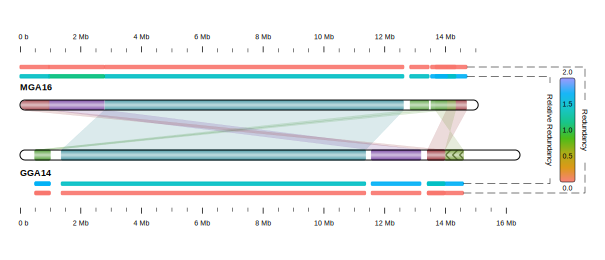
\includegraphics[width=.85\linewidth]{fig/GGA14_MGA16.pdf}
%   \caption{\textit{G.~gallus} chromosome~14 compared to \textit{M.~gallopavo} chromosome~16.
%    (a)~Smash++, employing an FCM and an STMM with $k=14$ and~5, respectively. The blocks smaller than 400~Kb are discarded;
%    (b)~progressiveMauve, with LCB weight of~27424;
%    (c)~adopted from \cite{zhang2011comparative}. The box shows an inversion rearrangement; 
%    (d)~SynBrowser, with the resolution of~150~Kb.
%   }
%   \label{fig.supp.GGA14.MGA16}
% \end{figure}

% \clearpage
% \section{HS 12 compared to PT 12}
% \begin{figure}[!h]
%   \centering
%   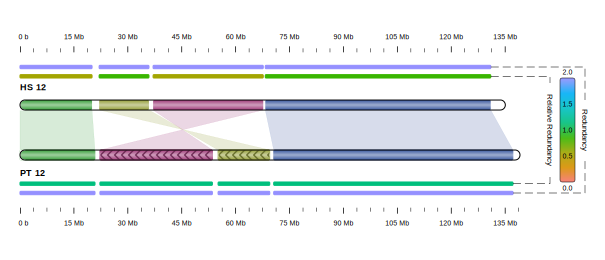
\includegraphics[width=.75\linewidth]{fig/HS12_PT12.pdf}
%   \caption{Comparison of \textit{H.~sapiens} chromosome~12 and \textit{P.~troglodytes} chromosome~12.
%    (a)~Smash++, with $k=14$ used by an FCM. The blocks smaller than 100~Kb are discarded;
%    (b)~progressiveMauve, with LCB weight of~55186;
%    (c)~Cinteny~\cite{sinha2007cinteny}, with minimum length of synteny block $=1~$Kb, maximum gap between adjacent markers $=5~$Mb and minimum number of markers $=1$;
%    (d)~SynBrowser, with the resolution of~150~Kb;
%    (e)~D-Genies~\cite{cabanettes2018d}, in ``strong precision'' mode.
%   }
%   \label{fig.supp.HS12.PT12}
% \end{figure}

% \clearpage
% \section{PXO99A compared to MAFF 311018}
% \begin{figure}[!h]
%   \centering
%   \includegraphics[width=\linewidth]{fig/PXO99A_MAFF311018.pdf}
%     \caption{Pair-wise comparison of PXO99A and MAFF 311018.
%      (a)~Smash++, with k=13 used by an FCM. The blocks smaller than 10~Kb are discarded. In order to make the figure clearer, the shaded paths for connecting corresponding regions are not drawn;
%      (b)~progressiveMauve, with LCB weight of~3926;
%      (c)~adopted from~\cite{salzberg2008genome}, which employs an alignment-based method to obtain this dot plot. The blue and red colors shows regions of PXO99A that align to the same or opposite strand of MAFF 311018, respectively.
%     }
%     \label{fig.supp.PXO99A.MAFF_311018}
% \end{figure}

% \clearpage
% \section{Tool availability and implementation}
% \label{sec.tool}
% \smashpp is implemented in \cpp language and is publicly available at~\cite{web-smashpp}, under GNU GPL~v3 license. This tool is able to find and visualize rearrangements in a pair of DNA sequences. It is recommended to use as input bare sequences, i.e., without header or quality scores, although, \fasta and \fastq formats are also supported. In the following sections, we describe installing and running the \smashpp tool.

% \subsection{Install}
% To install \smashpp on various operating systems, follow the instructions below. Note that the precompiled executables are available for 64 bit operating systems in the ``bin/'' directory.

% \subsubsection*{Conda}
% \begin{code}[style=bash]
%   conda install -c cobilab smashpp
% \end{code}

% \subsubsection*{Linux}
% \begin{itemize}
%   \item Install ``git'' and ``cmake'':
% \begin{code}[style=bash]
% sudo apt update
% sudo apt install git cmake
% \end{code}
% \item Clone \smashpp and install it:
% \begin{code}[style=bash]
% git clone https://github.com/smortezah/smashpp.git
% cd smashpp
% ./install.sh
% \end{code}
% \end{itemize}

% \subsubsection*{macOS}
% \begin{itemize}
%     \item Install ``Homebrew'', ``git'' and ``cmake'':
% \begin{code}[style=bash]
% /usr/bin/ruby -e "$(curl -fsSL https://raw.githubusercontent.com/Homebrew/install/master/install)"
% brew install git cmake
% \end{code}
% \item Clone \smashpp and install it:
% \begin{code}[style=bash]
% git clone https://github.com/smortezah/smashpp.git
% cd smashpp
% ./install.sh
% \end{code}
% \end{itemize}

% \subsubsection*{Windows}
% \begin{itemize}
%   \item Download and install ``CMake'', e.g., from https://github.com/Kitware/CMake/releases/\linebreak download/v3.14.4/cmake-3.14.4-win64-x64.msi. Make sure to add it to the system PATH. For example, if CMake is installed in ``C:\textbackslash Program Files'', add ``C:\textbackslash Program Files\textbackslash CMake\textbackslash bin'' to the system PATH.
%   \item Download and install ``mingw-w64'', e.g., from https://sourceforge.net/projects/mingw-w64/\linebreak files/latest/download. Make sure to add it to the system PATH. For example, if it is installed in ``C:\textbackslash mingw-w64'', add ``C:\textbackslash mingw-w64\textbackslash mingw64\textbackslash bin'' to the system PATH.
%   \item Download and install ``git'', from https://git-scm.com/download/win.
%   \item Clone \smashpp and install it:
% \begin{code}[style=bash]
% git clone https://github.com/smortezah/smashpp.git
% cd smashpp
% .\install.bat
% \end{code}
% \end{itemize}

% \subsection{Run \smashpp}
% Various options are provided with the interface of the proposed tool, which are described in Table~\ref{tab.options}. The commands for running \smashpp have the form of the following:
% \begin{code}[style=bash]
% ./smashpp [OPTIONS]  -r <REF-FILE>  -t <TAR-FILE>
% \end{code}

% \DeclareRobustCommand{\default}[1]{\hspace*{0mm}\colorbox{lightgray!30}{\footnotesize Default: #1}}
% \DeclareRobustCommand{\defaultbox}[1]{\colorbox{lightgray!30}{\footnotesize #1}}

% \begin{small}
% \begin{tabularx}{\linewidth}{@{}lp{2.9cm}X@{}}
%   \caption{Options provided by \smashpp interface.}
%   \label{tab.options} \\
%   \toprule
%   Flag & Input & Description \\
%   \midrule
%   \multicolumn{3}{@{}l@{}}{\textit{Required}} \\
%   \mono{-r} & Seq/FASTA/FASTQ & Reference file. Spaces in the name is supported. \\
%   \mono{-t} & Seq/FASTA/FASTQ & Target file. Spaces in the name is supported. \\
%   && It is recommended to have short names. \\
%   \midrule
%   \multicolumn{3}{@{}l@{}}{\textit{Optional}} \\
%   \mono{-l} & Integer: $[0, 6]$\newline \default{3} & Level of compression. \\
%   \midrule
%   \mono{-m} & Integer: $[1, 2^{32}-1]$\newline \default{50} & Minimum segment size. Only the regions that have greater sizes than this value would be considered for compression. \\
%   \midrule
%   \mono{-e} & Float: $[0.0, 100.0]$\newline \default{2.0} & Entropy of `N' bases. In implementation of the reference-based compression, we replace `N's in references and targets with `A's and `T's, respectively. On reference-free compression, we replace them with `A's, in both references and targets. If a user tends to replace `N' bases in a sequence with a normal distribution of `A', `C', `G' and `T's, he/she can employ GOOSE toolkit~\cite{web-goose}. \\
%   \midrule
%   \mono{-n} & Integer: $[1, 255]$\newline \default{4} & Number of threads. Creating multiple finite-context models and substitution-tolerant Markov models can be done in a multi-threaded fashion. \\
%   \midrule
%   \mono{-f} & Integer: $[1, 2^{32}-1]$\newline \default{256} & Filter size. In the process of finding similar regions in the reference and the target sequences, the information content that would be obtained by compression needs to be filtered. \\
%   \midrule
%   \mono{-ft} & Integer or String:\newline \{0/rectangular, 1/hamming, 2/hann, 3/blackman, 4/triangular, 5/welch, 6/sine, 7/nuttall\}\newline \default{hann} & Filter type (windowing function). Besides Hann window that is used by default to smooth the information content (profile), we have implemented several other windowing functions: Blackman~\cite{blackman1959particular}, Hamming~\cite{tukey1949measuring}, Nuttall~\cite{nuttall1981some}, rectangular~\cite{oppenheim1999discrete}, sine~\cite{harris1978use}, triangular~\cite{bartlett1950periodogram} and Welch~\cite{welch1967use} windows. These functions along with Hann function are given by Equation~\ref{eq.filter} and are plotted in Fig.~\ref{fig.filters}. \\
%   \midrule
%   \mono{-fs} & Char or String:\newline \{S/small, M/medium, L/large\}
%   % \newline Default: large
%    & Filter scale. It automatically chooses filter size. If a user does not use this flag, the ``-f'' flag will handle the filtering size.  \\
%   \midrule
%   \mono{-d} & Integer: $[1, 2^{64}-1]$ & Sampling steps. Instead of considering the whole information content, we can make samples of it. The default value is $\lceil\min\left(\lvert\textrm{ref}\rvert, \lvert\textrm{tar}\rvert\right) /\, 5000\rceil$. Therefore, if this flag is not entered by user, a maximum number of 5000 values of the information content will be considered. \\
%   \midrule
%   \mono{-th} & Float: $[0.0, 20.0]$\newline \default{1.5} & Threshold for entropy. This option can be used for segmenting the filtered information content. \\
%   % For the purpose of segmenting the filtered information content, the average entropy of reference-based compression is used by default as the threshold, but the threshold can be altered by this option. \\
%   \midrule
%   \mono{-rb} & Integer: $[-2^{15}, 2^{15}-1]$ & Reference beginning guard. \\
%   \mono{-re} & Integer: $[-2^{15}, 2^{15}-1]$ & Reference ending guard. \\
%   \mono{-tb} & Integer: $[-2^{15}, 2^{15}-1]$ & Target beginning guard. \\
%   \mono{-te} & Integer: $[-2^{15}, 2^{15}-1]$ & Target ending guard. \\
%   & \default{0} & \smashpp is capable of finding even very small similar regions in two sequences. However, we have found experimentally that when it is running in a very sensitive mode, there might be some cases in which the size of similar regions in the reference and the target are not balanced. These cases can be handled by ``-rb'', ``-re'', ``-tb'' and ``-te'' options, by resizing the beginning and ending guards of reference and target regions, respectively. For example, if ``-tb 10'' is used, the first 10 bases in each target region will be discarded, which results in smaller regions. Note that when the guard sizes of target regions are increased, the models built from these regions would be slightly different than the original models; consequently, the sizes of reference regions that are detected as being similar to the ones from the target would be altered. Therefore, changing the guard sizes of target regions will affect the sizes of reference regions. 
%   % In the case of activating deep compression, by ``-dp'', changing the guard sizes of reference regions would affect the sizes of target regions, as well.
%   The same thing happens for the sizes of target regions, when the guard sizes of reference regions are changed. \\
%   \midrule
%   \mono{-ar} & N/A & Consider asymmetric regions. It makes \smashpp not to balance the similar reference and target regions. \\
%   % \midrule
%   % \mono{-dp} & N/A & Deep compression. It means that similar regions in target and reference sequences are found in three phases, instead of two: 1)~the reference model is built and the target is compressed based upon that model, 2)~the model of each detected region is built and the whole reference is compressed based on those models and 3)~the model of each detected reference region is built and the corresponding target regions will be compressed based on that model. \\
%   \midrule
%   \mono{-nr} & N/A & Do not compute self complexity. It makes the tool not to perform the reference-free compression (self-complexity computation). \\
%   \midrule
%   \mono{-sb} & N/A & Save sequence (input: FASTA/FASTQ). \smashpp accepts as input \fasta and \fastq files, in addition to bare sequences. In these cases, the input files are first converted to sequences and then processed further. It is possible to save these sequences by this option. \\
%   \midrule
%   \mono{-sp} & N/A & Save profile, *.prf. When the information profile is obtained, \smashpp smoothens then removes it, by default; however, it can be preserved by this option. \\
%   \midrule
%   \mono{-sf} & N/A & Save filtered file, *.fil. The filtered profile is segmented then removed, by default; however, it can be preserved by this option. \\
%   \midrule
%   \mono{-ss} & N/A & Save segmented files, *.s$_i$. \\
%   \midrule
%   \mono{-sa} & N/A & Save all generated files, including profile, filtered and segmented files. \\
%   \midrule
%   \mono{-rm} & $k$,[$w$,$d$,]ir,$\alpha$,$\gamma$/$t$,ir,$\alpha$,$\gamma$:... & Parameters of reference models. \\
%   \mono{-tm} & $k$,[$w$,$d$,]ir,$\alpha$,$\gamma$/$t$,ir,$\alpha$,$\gamma$:... & Parameters of target models: \\
% & \default{}\newline\defaultbox{\scalebox{0.75}{$14,0,0.001,0.95/5,0,0.001,0.95$}}
%  & \begin{minipage} [t] {9cm}
%   \begin{itemize}
%     \item $k$ (integer $>1$): context size,
%     \item $w$ (integer $<2^{64}-1$): Count-Min-Log sketch width in $\log_2$ form, e.g., set 10 for $w=2^{10}=1024$,
%     \item $d$ (integer $>0$): Count-Min-Log sketch depth,
%     \item ir (integer: \{0, 1, 2\}): inverted repeat, including 0:~regular (not inverted), 1:~inverted solely, and 2:~both regular and inverted,
%     \item $\alpha$ (float $>0$): estimator,
%     \item $\gamma$ (float: $[0.0, 1.0)$): forgetting factor,
%     \item $t$ (integer $>0$): threshold (number of substitutions).
%   \end{itemize}
% \end{minipage} \\
%   && It is recommended for compression to use ``-l'' option, since it configures the models automatically. However, using ``-rm'' and ``-tm'', the user would be able to manually configure the reference model, for reference-based compression, and the target model, for reference-free compression, respectively. Parameters of models are described in detail in the section ``Methods'' of the main paper. \\
%   \midrule
%   \mono{-ll} & N/A & List of compression levels. It shows the list of parameters that would be chosen automatically for each model. \\
%   \midrule
%   \mono{-h} & N/A & Usage guide. \\
%   \midrule
%   \mono{-v} & N/A & More information (verbose). \\
%   \midrule
%   \multicolumn{2}{@{}l}{\mono{--version}} & Show the version. \\
%   \bottomrule
% \end{tabularx}
% \end{small}

% \begin{align}
%   w[n] & = 1,
%   \tag*{\small(rectangular)} \\
%   w[n] & = 0.54348-0.45652\;\cos \left(\tfrac {2\pi n}{N}\right),
%   \tag*{\small(Hamming)} \\
%   w[n] & = \sin^2 \left(\tfrac {\pi n}{N}\right),
%   \tag*{\small(Hann)} \\
%   w[n] & = 0.42659-0.49656\;\cos \left(\tfrac {2\pi n}{N}\right)+0.07685\;\cos \left(\tfrac {4\pi n}{N}\right),
%   \tag*{\small(Blackman)} \\
%   w[n] & = 1-\left|\tfrac {n-N/2}{N/2}\right|,
%   \tag*{\small(triangular/Bartlett)} \\
%   w[n] & = 1-\left(\tfrac {n-N/2}{N/2}\right)^{2},
%   \tag*{\small(Welch)} \\
%   w[n] & = \sin \left(\tfrac {\pi n}{N}\right),
%   \tag*{\small(sine)} \\
%   w[n] & = 0.35577-0.48740\;\cos \left(\tfrac {2\pi n}{N}\right)+0.14423\;\cos \left(\tfrac {4\pi n}{N}\right)-0.01260\;\cos \left(\tfrac {6\pi n}{N}\right),
%   \tag*{\small(Nuttall)} \\
%   \label{eq.filter}
% \end{align}

% \begin{figure}[!h]
%   \centering
%   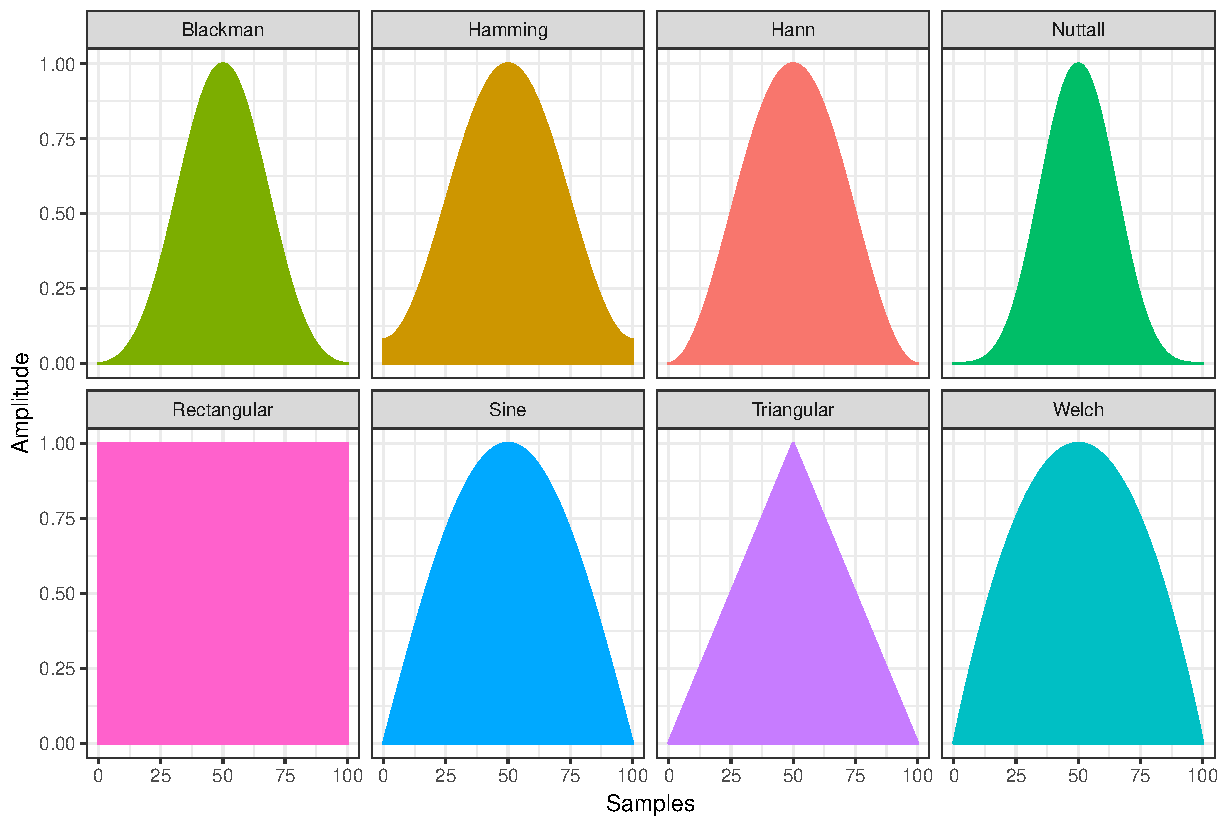
\includegraphics[width=.9\linewidth]{fig/filters.pdf}
%   \caption{Various windowing functions embedded in \smashpp.}
%   \label{fig.filters}
% \end{figure}

% By running \smashpp, positions of similar regions in reference and target sequences, relative redundancy and also redundancy (complexity) of the regions is saved in a ``.pos'' file. This tab-delimited file has a header including:
% \begin{enumerate}
%   \item The string ``\#\#SMASH++'' as a specifier for the \smashpp tool,
%   \item The ``PARAM'' line to list the parameters used to generate the position file,
%   \item The ``INFO'' line to provide the names and sizes of reference and target sequences,
%   \item The line with the names of columns of the body,
% \end{enumerate}
% and a body including:
% \begin{enumerate}
%   \item RBeg (Reference Begin): beginning of a reference region,
%   \item REnd (Reference End): end of a reference region,
%   \item RRelRdn (Reference Relative Redundancy): relative redundancy obtained by compressing the associated target block considering as reference this reference block,
%   \item RRdn (Reference Redundancy): redundancy (Complexity) of the detected reference block, calculated by reference-free compression,
%   \item TBeg (Target Begin): beginning of a target region,
%   \item TEnd (Target End): end of a target region,
%   \item TRelRdn (Target Relative Redundancy): relative redundancy obtained by compressing the associated reference block considering as reference this target block,
%   \item TRdn (Target Redundancy): redundancy (Complexity) of the detected target block, calculated by reference-free compression,
%   \item Inv (Invereted repeat): if the corresponding line is an inverted repeat. ``F''~(False) means it is regular and ``T''~(True) means it is inverted.
% \end{enumerate}
% As an example, the header of the following ``.pos'' file shows that \smashpp was run by the parameters ``-r dataset/REF -t dataset/TAR -l 0 -m 1000'' and also the reference ``REF'' and the target ``TAR'' are 50,000 base long. The body shows that there is a reference block, from the position 5000 up to 10000, similar to a target block, from the position 2000 to 7000. Relative redundancy of compressing the TAR block, using the REF block as reference, is 1.2473. This number is 1.0187 when the REF block is compressed based on the model of the TAR block. Also, redundancies (complexities) of the REF and the TAR blocks are 1.9010 and 1.8580, respectively. The ``F'' in the last column shows that this similarity is not of the form inverted repeat. The second record of the body shows an inverted repeat rearrangement.
% \begin{code}[style=bash]
% ##SMASH++
% ##PARAM=<-r dataset/REF -t dataset/TAR -l 1 -m 1000>
% ##INFO=<Ref=REF,RefSize=50000,Tar=TAR,TarSize=50000>
% #RBeg  REnd   RRelRdn  RRdn    TBeg   TEnd   TRelRdn  TRdn    Inv
% 5000   10000  1.0187   1.9010  2000   7000   1.2473   1.8580  F
% 20000  30000  1.2367   1.9777  40000  30000  1.2545   1.9888  T
% \end{code}

% \subsection{Run \smashpp visualizer}
% The position file obtained by \smashpp can be visualized by
% \begin{code}[style=bash]
% ./smashpp -viz
% \end{code}
% The visualizer provides various options that are described in Table~\ref{tab.options.viz}. The commands for running \smashpp visualizer are of the form
% \begin{code}[style=bash]
% ./smashpp -viz [OPTIONS]  -o <SVG-FILE>  <POS-FILE>
% \end{code}

% \begin{small}
%   \begin{tabularx}{\linewidth}{@{}lp{2.4cm}X@{}}
%     \caption{Options provided by \smashpp visualizer interface.}
%     \label{tab.options.viz} \\
%     \toprule
%     Flag & Input & Description \\
%     \midrule
%     \multicolumn{3}{@{}l@{}}{\textit{Required}} \\
%     & *.pos file & Position file, generated by \smashpp tool. Spaces in the name is supported. It can be redirected to \smashpp by standard input (``stdin''). \\
%     \midrule
%     \multicolumn{3}{@{}l@{}}{\textit{Optional}} \\
%     \mono{-o} & *.svg file\newline \default{map.svg} & Output image name. \\
%     \midrule
%     \mono{-rn} & String & Reference name shown on output. \\
%     \mono{-tn} & String & Target name shown on output. \\
%     & \default{names in}\newline\defaultbox{position file's header} & If it has some spaces, use double quotes, e.g. ``Seq label''. \\
%     \midrule
%     \mono{-l} & Integer: $[1, 6]$\newline \default{1} & Type of the link between similar regions. \\
%     \midrule
%     \mono{-c} & Integer: $[0, 1]$\newline \default{0} & Color mode. \\
%     \midrule
%     \mono{-p} & Float: $[0.0, 1.0]$\newline \default{0.9} & Opacity. \\
%     \midrule
%     \mono{-w} & Integer: $[8, 100]$\newline \default{10} & Width of the sequence. \\
%     \midrule
%     \mono{-s} & Integer: $[5, 200]$\newline \default{40} & Space between sequences. \\
%     \midrule
%     \mono{-tc} & Integer: $[1, 255]$ & Total number of colors in the map, which is automatically chosen by default. \\
%     \midrule
%     \mono{-rt} & Integer: $[1, 2^{32}-1]$ & Reference tick size. \\
%     \mono{-tt} & Integer: $[1, 2^{32}-1]$ & Target tick size. \\
%     \midrule
%     \mono{-th} & Integer: $\{0, 1\}$\newline \default{1} & Tick human readable: 0=false, 1=true. If it is true, the sizes on axes are printed in the format 1K, 2M, etc. Note that here, 1K is equivalent to 1000 and not 1024, and so on. \\
%     \midrule
%     \mono{-m} & Integer: $[1, 2^{32}-1]$\newline \default{1} & Minimum block size. Only the regions with greater sizes than this value will be illustrated. \\
%     \midrule
%     \mono{-vv} & N/A & Vertical view of the output image. \\
%     \midrule
%     \mono{-nn} & N/A & Do not show normalized relative compression (NRC). \\
%     \mono{-nr} & N/A & Do not show redundancy (self complexity). \\
%     && \smashpp performs reference-based and reference-free compressions to calculate the NRC and redundancy, respectively. If a user does not tend to show them, he/she can turn them off by ``-nn'' and ``-nr'' triggers. \\
%     \midrule
%     \mono{-ni} & N/A & Do not show inverse maps. \\
%     \mono{-ng} & N/A & Do not show regular (not inverse) maps. \\
%     && \smashpp considers by default both regular and reverse complement maps in its calculations. \\
%     \midrule
%     \mono{-h} & N/A & Usage guide. \\
%     \midrule
%     \mono{-v} & N/A & More information (verbose). \\
%     \midrule
%     \multicolumn{2}{@{}l@{}}{\mono{--version}} & Show version. \\
%     \bottomrule
%   \end{tabularx}
% \end{small}


\subsection{Example}
This section guides step-by-step employing \smashpp to find and visualize rearrangements between two synthetic sequences. Note that the commands can be run on Linux and macOS, however, they are similar in Windows.

% \subsubsection*{Install \smashpp and provide the required files}
First, install \smashpp:
\begin{code}[style=bash]
git clone https://github.com/smortezah/smashpp.git
cd smashpp
./install.sh
\end{code}
Then, copy ``smashpp'' executable file into ``example/'' directory and go to that directory:
\begin{code}[style=bash]
cp smashpp example/
cd example/
\end{code}
There is a 1000 byte reference sequence, named ``ref'', as the following:
\begin{verbatim}
TCCCGGTCTTTTAGCGGCCAGGGGCCTGGGCTGTATATCGAAAAGTAATATCCCTTTATGCACCGACCGTAATTATGGACAGCAC
ATATACATTATGAGATTTAAAGATCGCGTGGACGACCACGCGGGCTTATAGCCTCACCTGAGGAAGGGGGTGCCTGCGAGGGAGC
TTGAACCTGTAGCCCCAATCTCGAACGACCTGAGGCTTGTGTGGTCAGAGTTGTGACCAGAGCGATCCCGTTGTCAAATCAACCT
AGAGGAGAGGTAAGGGATACGGGTTACATCTCTCCGCTCAGATTGCTCCTATCGGTAGGAAATATCGGGGATAACCCAATACAAA
ACGCTGAACTGTTCATATTTAGCAAGAAGGGGGGACCGAGGAGCTAAATCAGGGACTATGTAAAATTAGAGTTCTAAGGATAGTA
GCACCCGCGCATGGATCGAACTCCGCCTTGGTTGGGTGTGGATGCCATTGGCGTCACCGTGCTGATAGCCAAATCCCTAGTGAAG
GTAACGTGCGGCCAATTAAATAGTAACTGGGCGTAGATTCTAGCGGTGGCCTCATACGGCACCAATGTCCATCCTCCCTGTGCCT
AACACTATAACTCCAATCCCGTGAGTCTACCATCGCCGAGAATCAGACGGGCAACAAACCCAGGGAGCGAGAGCTACGCGGCTTA
TATCACGGATGCTTCCCCACCTAGGGAAATTTGTTCCGCCTAATCCCGTCCTTCGCTGGTCAGGCCCGGTCTAGCGGATTACTTC
GCCGGTAATGCAGTACAGAATAAATGAAATTCATTAAGAGAATGAAAGGTTATCAGCGAAGCCTTAAGGTCCAACAAGACGTCGA
TATTCTGAAGTAAACTGGTTGACATGTGTGTAACATGAAGCACGCGCTTATTGATATTATCCGCAACCCCACGGCTGGCGGGAAT
CAACCGGCGTCCAGTTCGAACAAGACAGTGCGCTACGCATTACGAAATAGGCTTCGTGTTGCTGT
\end{verbatim}
and a 1000 byte target sequence, named ``tar'', in this directory:
\begin{verbatim}
CAGCAACACGAAGCCTATTTCGTAATGCGTAGCGCACTGTCTTGTTCGAACTGGACGCCGGTTGATTCCCGCCAGCCGTGGGGTT
GCGGATAATATCAATAAGCGCGTGCTTCATGTTACACACATGTCAACCAGTTTACTTCAGAATATCGACGTCTTGTTGGACCTTA
AGGCTTCGCTGATAACCTTTCATTCTCTTAATGAATTTCATTTATTCTGTACTGCATTACCGGCGAAGTAATCCGCTAGACCGGG
CCTGACCAGCGAAGGACGGGATTAGGCGGAACAAATTTCCCTAGGTGGGGAAGCATCCGTGATATAAGCCGCGTAGCTCTCGCTC
CCTGGGTTTGTTGCCCGTCTGATTCTCGGCGATGGTAGACTCACGGGATTGGAGTTATAGTGTTAGGCACAGGGAGGATGGACAT
TGGTGCCGTATGAGGCCACCGCTAGAATCTACGCCCAGTTACTATTTAATTGGCCGCACGTTACCTTCACTAGGATCCCGGTCTT
TTAGCGGCCAGGGGCCTGGGCTGTATATCGAAAAGTAATATCCCTTTATGCACCGACCGTAATTATGGACAGCACATATACATTA
TGAGATTTAAAGATCGCGTGGACGACCACGCGGGCTTATAGCCTCACCTGAGGAAGGGGGGGCCTGCGAGGGAGCTTGAACCTGT
AGCCCCAATCTCGAACGACCTGAGGCTTGTGTGGTCAGAGTGGTGACCAGAGCGATCCCGTTGTCAAATCAACCTAGAGGAGAGG
TAAGGGATACGGGTTACATCTCTCCGCTCAGATTGCTCCTATCGGTAGGAAATATCGGGGATAACCCAATACAAAACGCTGAACT
GTTCATATTTAGTAAGAACGGGTGACCGAGGAGCTAAATCAGGGACTATGTAAAATTAGAGATCTAAGGATAGTAGCACCCGCGC
ATGGATCGAACTCCGCCATGGTTTGGTGTCGATGCCATTGGCGTCACCGTGCTGATAGCCAAATC
\end{verbatim}



% \colorbox{lightgray!30}{\parbox{0.9\textwidth}{
%   CAGCAACACGAAGCCTATTTCGTAATGCGTAGCGCACTGTCTTGTTCGAACTGGACGCCGGTTGATTCCCGCCAGCCGTGGGGTT
% }
\begin{code}[]
CAGCAACACGAAGCCTATTTCGTAATGCGTAGCGCACTGTCTTGTTCGAACTGGACGCCGGTTGATTCCCGCCAGCCGTGGGGTT
\end{code}



Running
\begin{code}[style=bash]
./smashpp -r ref -t tar
./smashpp -viz -o example.svg ref.tar.pos
\end{code}
results in Fig.~\ref{fig.example}.

\begin{figure}[!h]
  \centering
  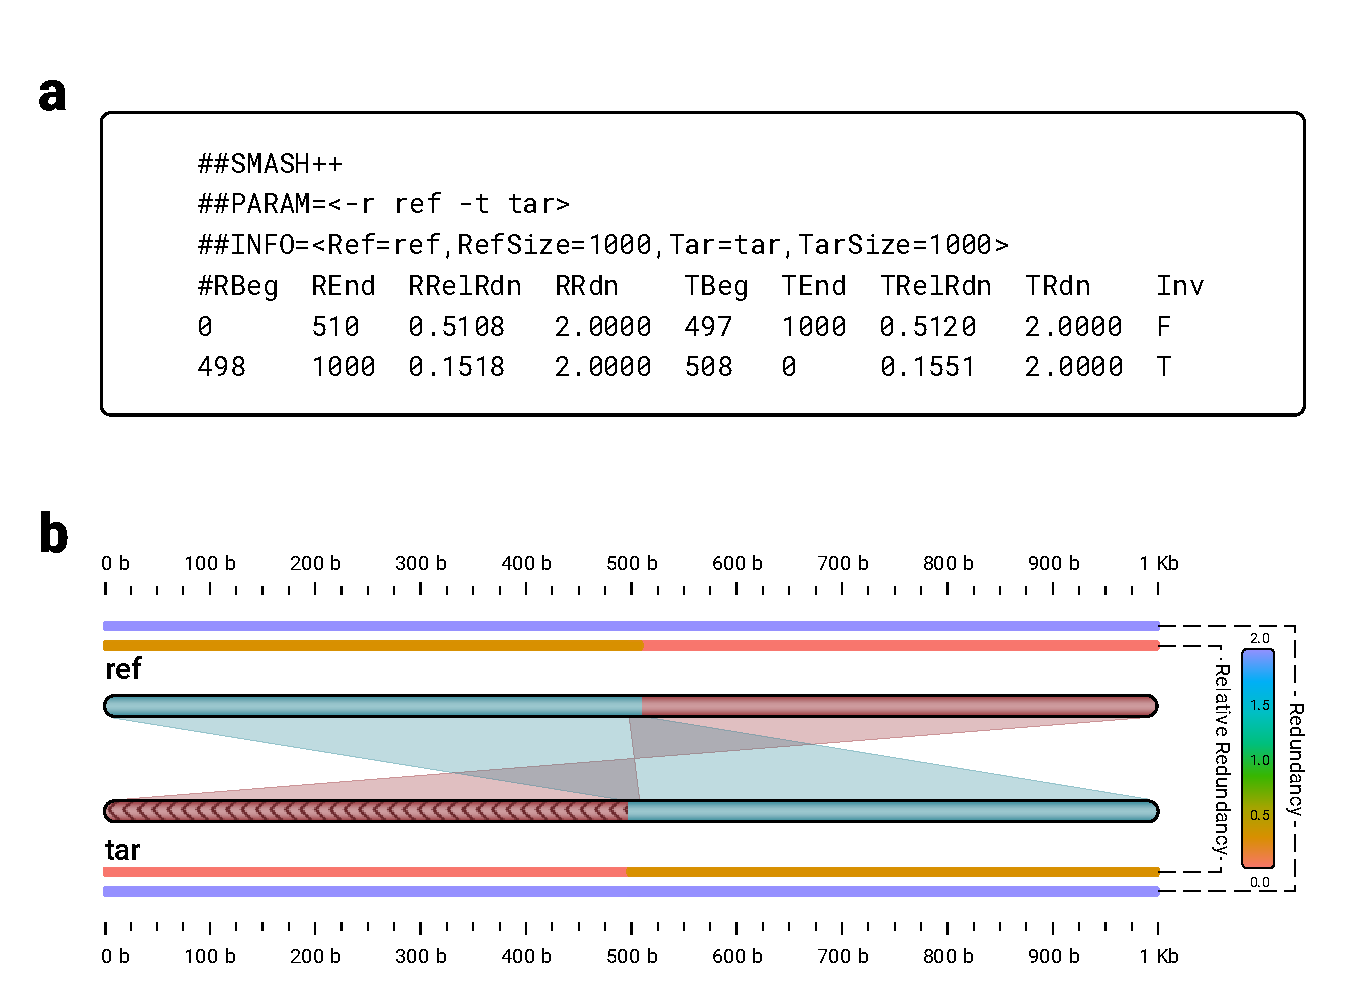
\includegraphics[width=.75\linewidth]{fig/example.pdf}
  \caption{An example of running \smashpp on two 1000 base sequences. (a) the position file and (b) output of the visualizer. One similar region in regular mode and another similar region in inverted mode are detected.}
  \label{fig.example}
\end{figure}

\clearpage
%\balance
\refLineSpace    %%% Line spacing
\small
\addcontentsline{toc}{section}{\:\textbf{References}}
\bibliographystyle{IEEEtran}
\bibliography{ref}

\end{document}